\documentclass{article}%
\usepackage[T1]{fontenc}%
\usepackage[utf8]{inputenc}%
\usepackage{lmodern}%
\usepackage{textcomp}%
\usepackage{lastpage}%
\usepackage{parskip}%
\usepackage{geometry}%
\geometry{tmargin=2cm,lmargin=3cm}%
\usepackage{amsmath}%
\usepackage{graphicx}%
\usepackage{ragged2e}%
\usepackage{multirow}%
%
\title{Auto{-}generated Report for Softleg Jump}%
\author{Andrea Boscolo Camiletto e Marco Biasizzo}%
\date{\today}%
%
\begin{document}%
\normalsize%
\maketitle%
\section{Settings of the problem}%
\label{sec:Settingsoftheproblem}%
The problem to be solved is the jumping procedure of a SEA based leg.%
The time horizon is 0.04 sec, with a number of steps of 25. That results in an open loop control at 625.0 Hz.

%
\section{Results}%
\label{sec:Results}%
The vertical velocity of the leg, at the last timestep, is:%
\[%
\boldsymbol{0.0181\,\, m/s}%
\]%
Keep in mind that a good value may be between $0.5$ and $2.0 \, m/s$

%
\section{Cost Function}%
\label{sec:CostFunction}%


\begin{figure}[h!]%
\centering%
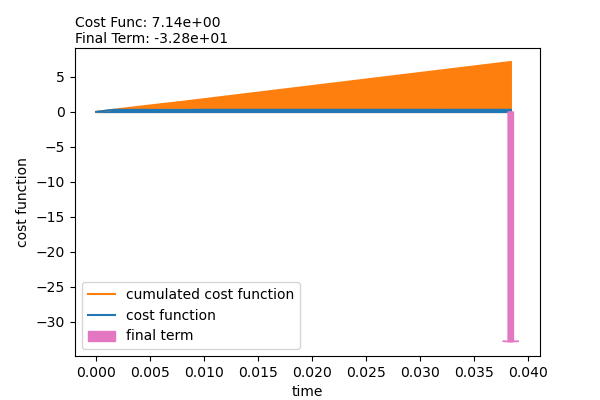
\includegraphics[width=250px]{/home/andrea/rob_project/softleg_jump/src/softleg-jump/script/trials/trial1/jump/visual/images/cost.png}%
\caption{Cost Function Analysis}%
\end{figure}

%
%
The values of the cost function and the final term cost are decently balanced, well done.

%
\pagebreak%
\section{Final Constraints}%
\label{sec:FinalConstraints}%
\begin{center}%
\begin{tabular}{c|c|c|c}%
\hline%
\multicolumn{4}{|c|}{Final Constraints Evaluation}\\%
\hline%
Constraint&Lower Bound&End Result&Upper Bound\\%
\hline%
&&&\\%
\multirow{1}{*}{vel\_x of CoM}&{-}0.0&0.0003&0.0\\%
\hline%
\multirow{1}{*}{pos\_x of CoM}&{-}0.0&{-}0.012&0.0\\%
\hline%
\multirow{1}{*}{vertical tip 1}&{-}0.0&0.0577&0.0\\%
\hline%
\end{tabular}%
\end{center}

%
\section{Joints Behaviour}%
\label{sec:JointsBehaviour}%


\begin{figure}[h!]%
\centering%
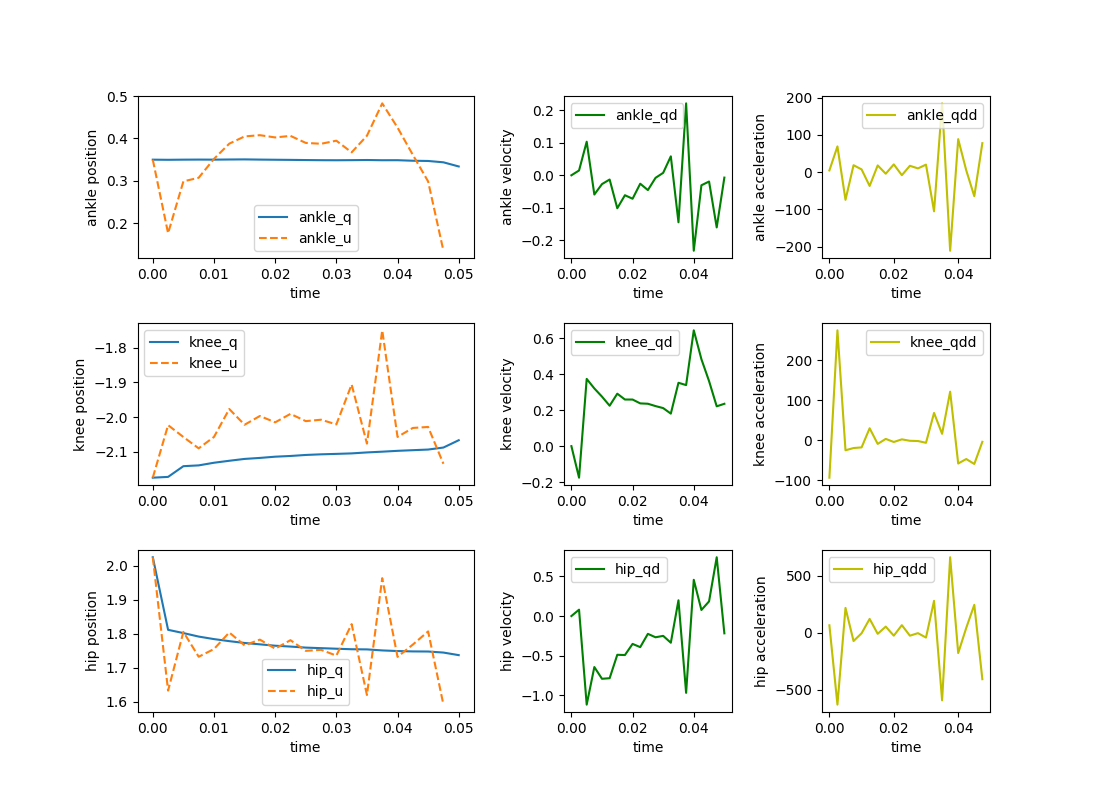
\includegraphics[width=400px]{/home/andrea/rob_project/softleg_jump/src/softleg-jump/script/trials/trial1/jump/visual/images/joints.png}%
\caption{Joints Dynamics}%
\end{figure}

%
On the figure above you can see on the rows the 3 joints and on the columns its position, velocity and acceleration.

%
\pagebreak%
\section{Constraints}%
\label{sec:Constraints}%


\begin{figure}[h!]%
\centering%
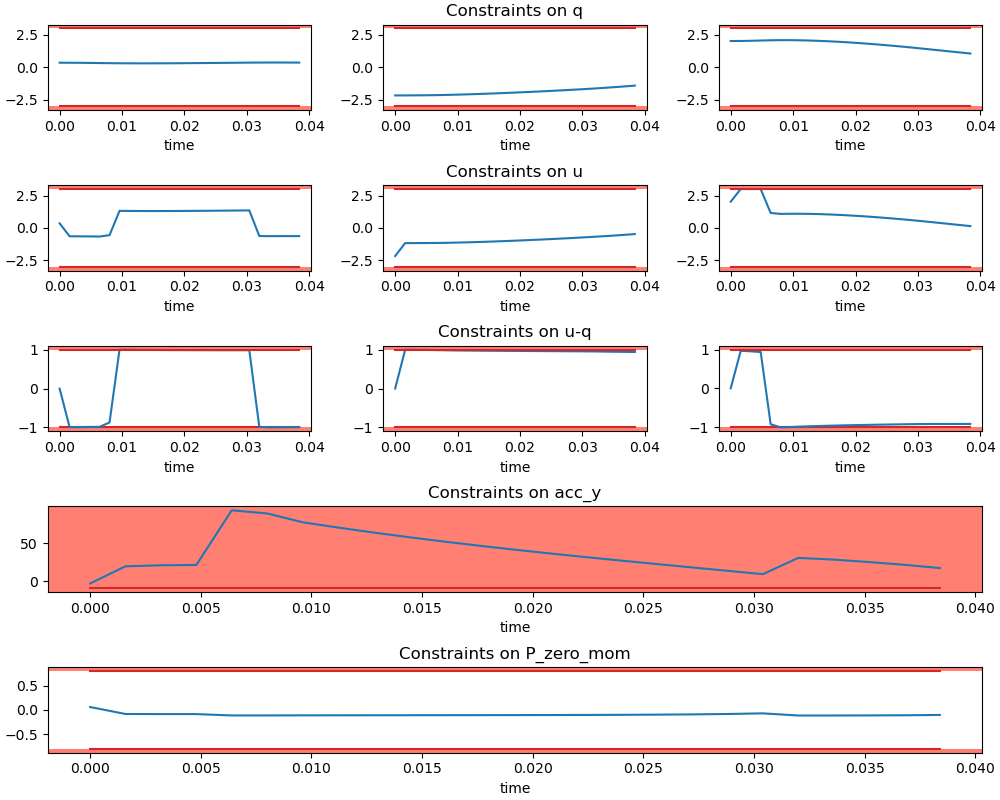
\includegraphics[width=400px]{/home/andrea/rob_project/softleg_jump/src/softleg-jump/script/trials/trial1/jump/visual/images/constr.png}%
\caption{Cost Function Analysis}%
\end{figure}

%
On the figure above you can see on the rows the different constraint, and on the column their plot per dimension. The titles are based on the configuration you set in the python file.

%
\end{document}